\documentclass{article}

\usepackage{tikz}
\usepackage{tkz-graph}
\usepackage{tkz-berge}

\begin{document}

Este es un ejemplo:
\begin{center}
  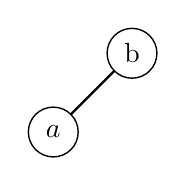
\begin{tikzpicture}
    \Vertex[x=0,y=0,Math]{a}
    \Vertex[x=1,y=1]{b}
    \Edge(a)(b)
  \end{tikzpicture}
\end{center}

\begin{center}
  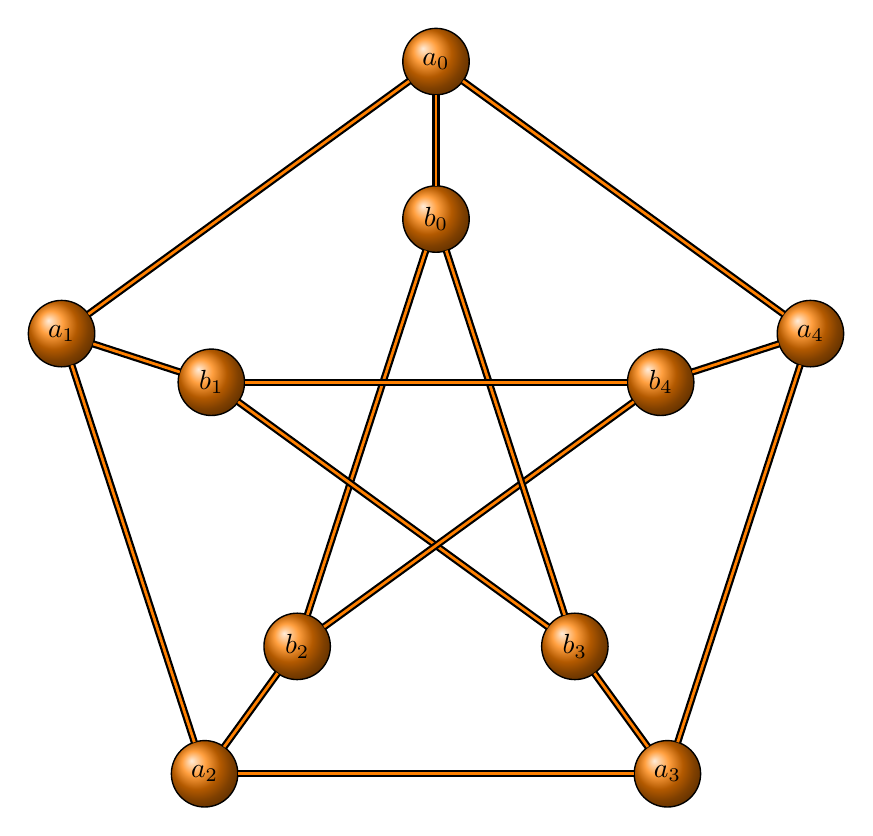
\begin{tikzpicture}
    \GraphInit[vstyle=Shade]
    %\GraphInit[vstyle=Art]
    %\SetVertexNoLabel
    \grPetersen[Math,rotation=90,RA=5,RB=3]
  \end{tikzpicture}
\end{center}

\end{document}
